\documentclass[12pt,fleqn]{article}\usepackage{../common}
\begin{document}
Dinamik Programlama

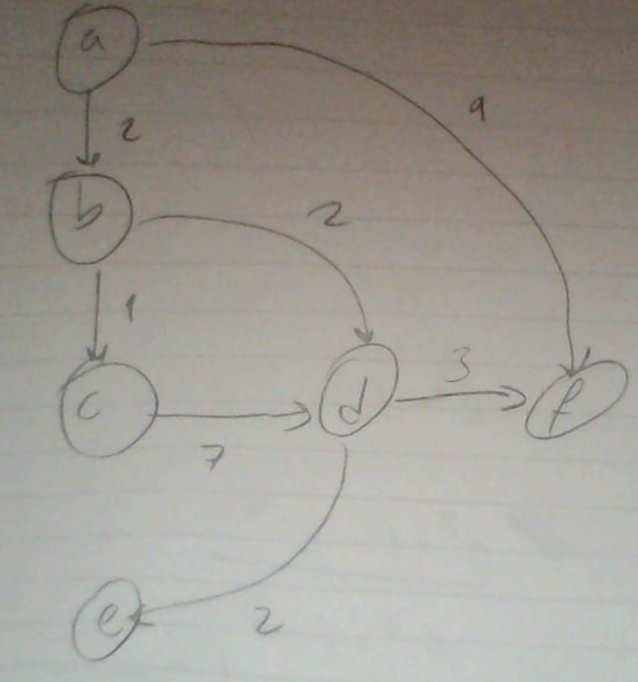
\includegraphics[height=6cm]{dp1.jpg}

Ustteki cizite tekabul eden veriyi kodlayalim

\begin{lstlisting}[language=Python]
DAG = {
    'a': {'b':2, 'f': 9},
    'b': {'d':2, 'c':1, 'f': 6},
    'c': {'d':7},
    'd': {'e':2, 'f': 3},
    'e': {'f':4},
    'f': {}
}
\end{lstlisting}

En kisa yolu bulacak program

\begin{lstlisting}[language=Python]
from functools import wraps

def memo(func):
    cache = {}                                  
    @wraps(func)                                
    def wrap(*args):                            
        if args not in cache:
            print 'miss', args
            cache[args] = func(*args)
        else: print 'hit', args
        return cache[args]                      
    return wrap 

def rec_dag_sp(W, s, t):                        
    @memo                                       
    def d(u):
        print ('in u')
        if u == t: return 0                     
        return min(W[u][v]+d(v) for v in W[u])  
    return d(s)                                 

dist = rec_dag_sp(DAG, 'a', 'f')
print 'uzaklik=', dist
\end{lstlisting}

\begin{verbatim}
miss ('a',)
in u
miss ('b',)
in u
miss ('c',)
in u
miss ('d',)
in u
miss ('e',)
in u
miss ('f',)
in u
hit ('f',)
hit ('d',)
hit ('f',)
hit ('f',)
uzaklik= 7
\end{verbatim}

\end{document}
